\chapter{State of the art}

\label{Chapter2}

\section{Overview of SCRUM and its challenges}
\subsection{Introduction to SCRUM}

In the ever-evolving landscape of project management and software development, 
one methodology has risen to the top as a new standard for agility, collaboration, 
and iterative progress - SCRUM. SCRUM, among other agile frameworks like XP\footnote{Extreme programming: \url{http://www.extremeprogramming.org/}} or Kanban\footnote{\url{https://www.ionos.com/digitalguide/websites/web-development/about-kanban/}} has become a pervasive framework employed by 
teams and organizations seeking a dynamic and responsive approach to complex projects. 
Its simplicity, adaptability, and focus on delivering value have made it a preferred 
choice in many economic sectors like software development 
and marketing \parencite{AgileTransformationSurvey}.

SCRUM emphasizes continuous learning and constant adaptation. 
It replaces traditional, linear project management approaches with an iterative, cyclic process. 

This section will include information about the SCRUM framework,
exploring the roles of the Scrum Master, Production Owner,
and Development Team members and how they work together to create and maintain projects. 
Moreover, the challenges that SCRUM teams often face and how they navigate these 
obstacles to deliver results will also be discussed. 

\subsection{Framework and Components}

At the heart of SCRUM lies a well-defined framework that serves as the blueprint for its application. This framework includes a set of interrelated components and processes. To understand SCRUM, it is essential to be acquainted with these fundamental elements \parencite{TheScrumGuide}.

\subsubsection*{Roles}

\begin{itemize}
    \item \textbf{SCRUM Master}: This role is dedicated to facilitating the SCRUM process, 
        ensuring that the team follows the SCRUM principles.
    \item \textbf{Product Owner}: The Product Owner represents the voice of the 
        customer and is responsible for defining and prioritizing items in the Product Backlog.
    \item \textbf{Development team}: The Development team is a self-organizing 
        group responsible for delivering the increments of work defined in the Sprint backlog
\end{itemize}

\subsubsection*{Product Backlog}

The product backlog stands as the repository of all future features, 
fixes, and requirements for the project. 
It's a dynamic list, constantly evolving to reflect changing priorities and market needs. 
The Product Owner is responsible for maintaining this backlog, 
ensuring that it aligns with the project's vision and objectives.

\subsubsection*{Time-boxed Sprints}
One of SCRUM's features is its reliance on time-boxed iterations known as Sprints.
Sprints are typically short, often lasting two to four weeks, 
during which the Development team focuses on delivering a 
potentially shippable product increment.

\subsubsection*{Sprint Backlog}

From the often very long Product Backlog, the team selects a subset of items 
to work on during a designated time period known as a Sprint.
These selected items form the Sprint Backlog. 
It is a commitment made by the Development Team for the duration of 
the Sprint and serves as a practical guide for their work.

\subsubsection*{Daily Standup}

SCRUM promotes daily collaboration and information sharing through the Daily Standup, 
a short and focused meeting where team members discuss their progress,
obstacles, and plans. 
This can enhance communication and keep everyone up to
date with the Sprint progress.

\subsubsection*{Sprint Review}

At the end of each Sprint, the team showcases the completed work to the
Product Owner and other relevant parties.
This event, known as the Sprint Review, provides an
opportunity for feedback and allows stakeholders to
inspect and adapt the product.

\subsubsection*{Sprint Retrospective}

After the Sprint Review, the team holds a meeting called Sprint
Retrospective to reflect on their performance and identify
areas for improvement. 
This meeting fosters a culture of continuous learning and adaptation.  

\subsection{Benefits}

SCRUM offers a myriad of benefits that have cemented its status as a
leading agile methodology in project management and software development.
The framework fosters agility and adaptability and 
aims to have many benefits for teams as stated in the official guide \parencite{TheScrumGuide}. 

Its iterative approach allows teams to respond swiftly to changing requirements
and market dynamics, ensuring that the end product remains aligned with evolving needs.
Moreover, SCRUM prioritizes transparency and collaboration,
encouraging open communication among team members and stakeholders.
This results in a shared understanding of project goals and progress, 
reducing the risk of misunderstandings or misalignments. 
SCRUM also emphasizes the delivery of value in each Sprint,
enabling teams to demonstrate results quickly, gather feedback,
and make necessary adjustments. This iterative process contributes to higher 
customer satisfaction and reduced time-to-market for products and solutions. 
This becomes evident by looking at popular surveys done for agile methods \parencite{AgileTransformationSurvey} \parencite{StateOfAgile2023}.

\subsection{Challenges}
Despite its numerous advantages, SCRUM does present some challenges.
One prominent challenge that many companies experience according to surveys 
lies in the cultural shift it requires \parencite{AgileTransformationSurvey}.
SCRUM fundamentally changes how teams work, demanding a shift from 
traditional command-and-control structures to self-organizing, cross-functional teams. 
This transition can be challenging and may encounter resistance within organizations. 
Another challenge is that SCRUM does not prescribe specific engineering practices, 
leaving it up to teams to determine their development methods.
While this flexibility is an asset, it can also lead to inconsistencies 
in quality and practices if not managed effectively.
Moreover, SCRUM's success is contingent on integrating with the product and the landscape 
the organization is building. This is a challenge today because teams may have ambitions to 
use agile methods like SCRUM but are hindered by their products.
To use data, 36\% of respondents of the agile transformation 
survey \textit{disagree} or \textit{strongly disagree} that their entire landscape 
was not suited for their agile ambition \parencite{AgileTransformationSurvey}.
Therefore, while SCRUM offers significant benefits, 
it necessitates a thoughtful and committed approach to overcome these challenges effectively.

\subsection{Measuring SCRUM's success}
Measuring SCRUM's success is a critical endeavor, and it can be accomplished through the use of KPIs.
KPIs offer a quantifiable and objective means to assess various facets of SCRUM implementation. 
An article published in 2023 \parencite{PercPerfOfMetrForAgileScrumEnv} discusses the perceived importance 
of SCRUM metrics. 
From this data it can be interpreted that the following KPIs are 
important for measuring a team's performance: Velocity, 
Accuracy of estimation, and Work capacity. Firstly, Velocity, a commonly used KPI in SCRUM, 
measures the rate at which a team delivers work, offering insights into its efficiency and productivity. 
Second, Accuracy of estimation describes how well the team did during its planning phase of the Sprint. 
And lastly, Work capacity describes how many resources the team had to begin with.

\newpage

\section{Previous studies and state of the art}\label{SOTAStudies}

When it comes to analyzing SCRUM processes, there are numerous software options available. 
The software a company chooses often depends on its prior investments in planning tools. 
Popular planning platforms like Jira Boards and Azure DevOps typically include basic analysis 
features as well.

\subsection{Relevant literature about KPIs and SCRUM Performance}

\subsubsection{Perceived Importance of Metrics for Agile Scrum Environments}

In a study published by Almeida and Carneiro in 2023 a survey about popular SCRUM metrics 
was conducted \parencite{PercPerfOfMetrForAgileScrumEnv}. 
The survey got 191 valid responses from 47 Product owners, 66 Scrum masters, 
and 78 members of development teams of which most had more than 2 years of experience with SCRUM. 
The survey asked participants to review different SCRUM metrics in each phase and activity of a sprint.
The metrics were rated on a scale of 1 to 5 where 5 indicates a high perceived importance 
of the metric by the participant. 
After data analysis and discussion of the results, some exact conclusions were made.


\begin{figure}[!th]
\centering
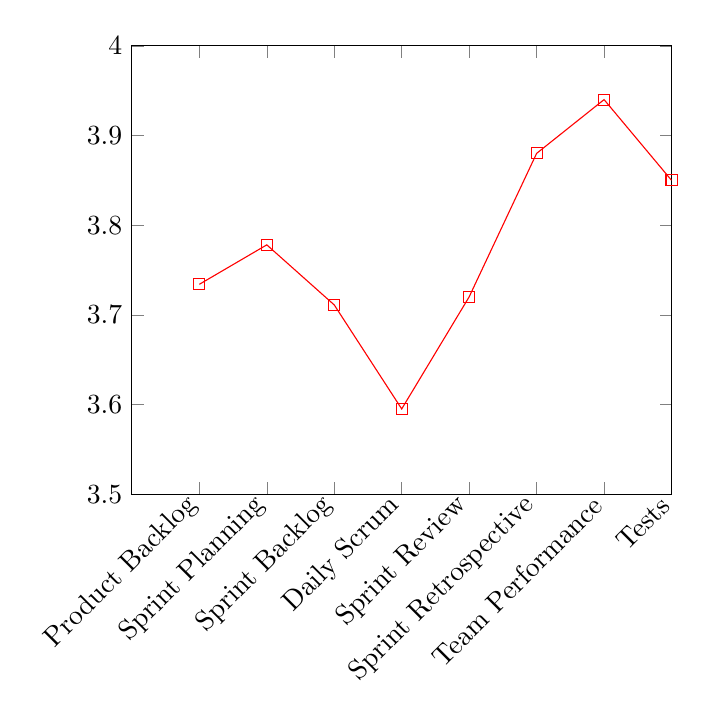
\begin{tikzpicture}
\begin{axis}[
    xmin=0, xmax=8,
    ymin=3.5, ymax=4,
    xtick=data,
    xticklabels={
        Product Backlog,
        Sprint Planning,
        Sprint Backlog,
        Daily Scrum,
        Sprint Review,
        Sprint Retrospective,
        Team Performance,
        Tests
    },
    x tick label style={rotate=45,anchor=east},
    legend pos=north west,
    grid style=dashed,
]
    
\addplot[
    color=red,
    mark=square,
]
coordinates {
    (1,3.734)
    (2,3.778)
    (3,3.711)
    (4,3.595)
    (5,3.72)
    (6,3.88)
    (7,3.94)
    (8,3.85)
};

\end{axis}
\end{tikzpicture}    
\decoRule
\caption[SCRUM metrics]{Scrum metric importance by activities, Source: \cite{PercPerfOfMetrForAgileScrumEnv}}
\label{fig:ScrumMetricsImportance}
\end{figure}

\noindent The figure (\ref{fig:ScrumMetricsImportance}) shows the mean of perceived importance 
of metrics that belong to a certain activity or category. 
From this one can conclude that me most important metrics are linked to 
team performance and the sprint retrospective.

\noindent The table \ref{tab:ScrumMetricsImportanceTable} illustrates the KPIs and their 
perceived importance within those categories. 
The mode represents the most frequent response given by the 
participants and the mean represents the mean value of all responses. In it's original form 
this table is quite large and was reduced to the KPIs relevant to this thesis. KPIs that were removed
were not relevant because they indicate performance in different SCRUM stages than planning and retrospective.
The aim of this thesis is to bring forth a method of evaluating SCRUM sprints automatically and only the KPIs listed 
in table \ref{tab:ScrumMetricsImportanceTable} were relevant for this stage of the process.


\begin{table}[]
    \centering
    \begin{tabular}{l l c c}
        \hline
        \textbf{Activity} & \textbf{Metric} & \textbf{Median} & \textbf{Mode} \\
        \hline
        Sprint backlog & Number of user stories & 4 & 5 \\
        & Number of tasks & 4 & 4 \\
        Sprint retrospective & Number of tasks in a sprint & 3 & 3 \\
        & Number of tasks completed in a sprint & 4 & 5 \\
        & Number of user stories completed in a sprint & 4 & 5 \\
        Team performance & Accuracy of estimation & 4 & 5 \\
        & Focus factor & 4 & 4 \\
        & Targeted value increase & 4 & 4 \\
        & Team member turnover & 4 & 3 \\
        & Team satisfaction & 4 & 4 \\
        & Velocity & 4 & 5 \\
        & Work capacity & 4 & 4 \\
    \end{tabular}
    \decoRule
    \caption[SCRUM metrics]{SCRUM metric importance by activities relevant to this thesis, Source: \cite{PercPerfOfMetrForAgileScrumEnv}}
    \label{tab:ScrumMetricsImportanceTable}
\end{table}

Based on the data, several conclusions can be made as a base for this thesis.
Both the number of completed tasks and the work done in story
points are crucial for a comprehensive sprint evaluation. 
Most metrics are objective and can be assessed without human intervention, 
with the exception of metrics like team satisfaction. 
The data also suggests that certain metrics, such as the number of 
planned user stories and tasks, 
should be determined before the sprint begins.

\subsubsection{Master thesis: Agile project health indicators}

In a master thesis published in 2019, Alexandra Esguerra states that 
performance indicators are essential for development and can be viewed as health checks for a project.
She lays out the challenges when selecting KPIs for a project and emphasizes that
the set of needed KPIs heavily depends on the team and the project itself.

A few different KPIs are mentioned and described as \textit{basis practices} in the analysis of agile methods in the following way:

\begin{itemize}
    \item \textbf{Velocity (Productivity)}: [...] You estimate this by defining the amount of completed user stories in very iteration. This measurement could help to estimate and see the overall productivity of the different teams.
    \item \textbf{Burn-down Chart}: This is a good tool to plan and monitor the progress in agile methods. It is also a way to show the remaining work. This [...] could be a guiding process to decision making on what to add or drop in case there is any delay on the project.
    \item \textbf{Schedule performance Indicator (SPI)}: This KPI will help to provide a clear view of the Schedule variance in the agile projects.
    \item \textbf{Cost performance indicator (CPI)}: This KPI will show how efficiently the project is spending the budget compared to how effectively it is planned to be spend.
\end{itemize}

The goal of the master thesis is to discover how KPIs can be applied in agile projects.
It also encourages readers to change traditional ways of thinking when it comes to project management
and shift to an agile mindset.

Some parts of this master thesis are also relevant to this bachelor thesis.
It can be learned that KPIs are essential in an agile context and that they depend 
heavily both on the project and the team that is using them.

\subsection{Non - academic articles}

This section includes some mentions of articles on the internet written by bloggers and companies.
While the intention behind these articles may be of educational nature it is important that the reader
is informed that they are not of academical origin and are to be taken with a grain of salt.

Nevertheless they are relevant to this thesis to further push the point that teams require a spectrum of different 
SCRUM KPIs that are tailored to their specific needs.

\subsubsection*{SCRUM Metrics 101 - Atlassan}

The article 'SCRUM Metrics 101' which was published by Erika Sa on the website 
\textit{atlassian.com} describes how SCRUM metrics can enhance the 
effectiveness of the process \parencite{Atlassian2023}. 
The article argues that these metrics are essential for making informed 
decisions during and after a sprint. 
The article also stresses that there is no universal set of 
metrics that can work for any team using SCRUM. 
Each team needs to choose metrics that are useful to their situation. 

Erika Sa also explains that SCRUM metrics can be a great indicator of 
erformance but should not be the sole ingredient to analyze a team's performance. 
Harder to comprehend numbers like customer satisfaction should also be considered to
get the full picture.

In summary, the article advocates for a balanced,
data-driven approach to SCRUM metrics. 
It discourages teams from relying on intuition or gut 
feeling to improve their performance. 
Instead, it promotes the use of specific metrics to 
bring various dimensions of a team's 
effectiveness to the surface. The mentioned metrics for 
this are velocity, capacity, and quality of output.

\subsubsection*{11 Scrum Metrics and Their Value to Scrum Teams}
This article describes SCRUM metrics and how they are evaluated, 
focusing only on the categories Sprint planning, Daily SCRUM, 
and Sprint Retrospective \parencite{Sealights2023}. 
It describes the goals of KPIs used in SCRUM to measure the value of products 
delivered by the team and the effectiveness of the method. According to this website, 
KPIs may also help catch problems like dissatisfied developers early.
The article selects 11 KPIs and describes how they are helpful in combination with using SCRUM. 
Four of those are relevant to this thesis as they capture values relevant to SCRUM sprints.

\begin{itemize}
    \item \textbf{Sprint Goal success}:
    This KPI indicates whether the planned sprint goal has been met or not. It's simple to evaluate and quickly points out how well the team did.

    \item \textbf{Escaped defects and defect density}:
    Escaped defects describe every bug or issue that is encountered by a user in production. Defect density is a metric that shows the number of defects relative to the software size. Software size is typically the number of lines in the code.

    \item \textbf{Team Velocity}:
    The number of tickets completed by a team during a sprint is an indicator of how much work got done. If this number is averaged over previous sprints the KPI Velocity is computed. A rise in Velocity may indicate an increase in productivity.

    \item \textbf{Sprint Burndown}:
    The sprint burndown chart shows if the team is on schedule to complete the sprint or not. It shows the ideal trend line of the completed work for each day in comparison to the actual completed work.

\end{itemize}

Other metrics mentioned in the article are Time to Market, ROI, and Customer Satisfaction. Most of those are irrelevant for this thesis as they are not evaluated on each Sprint and therefore have no impact on improving performance sprint to sprint. Others like Team Satisfaction and Team Member Turnover do not apply as well because they are not objective numbers that can be computed and used as a solid base for performance evaluation.

